\documentclass[tikz,border=10pt]{standalone}
\usepackage{tikz}
\usetikzlibrary{positioning}

\begin{document}
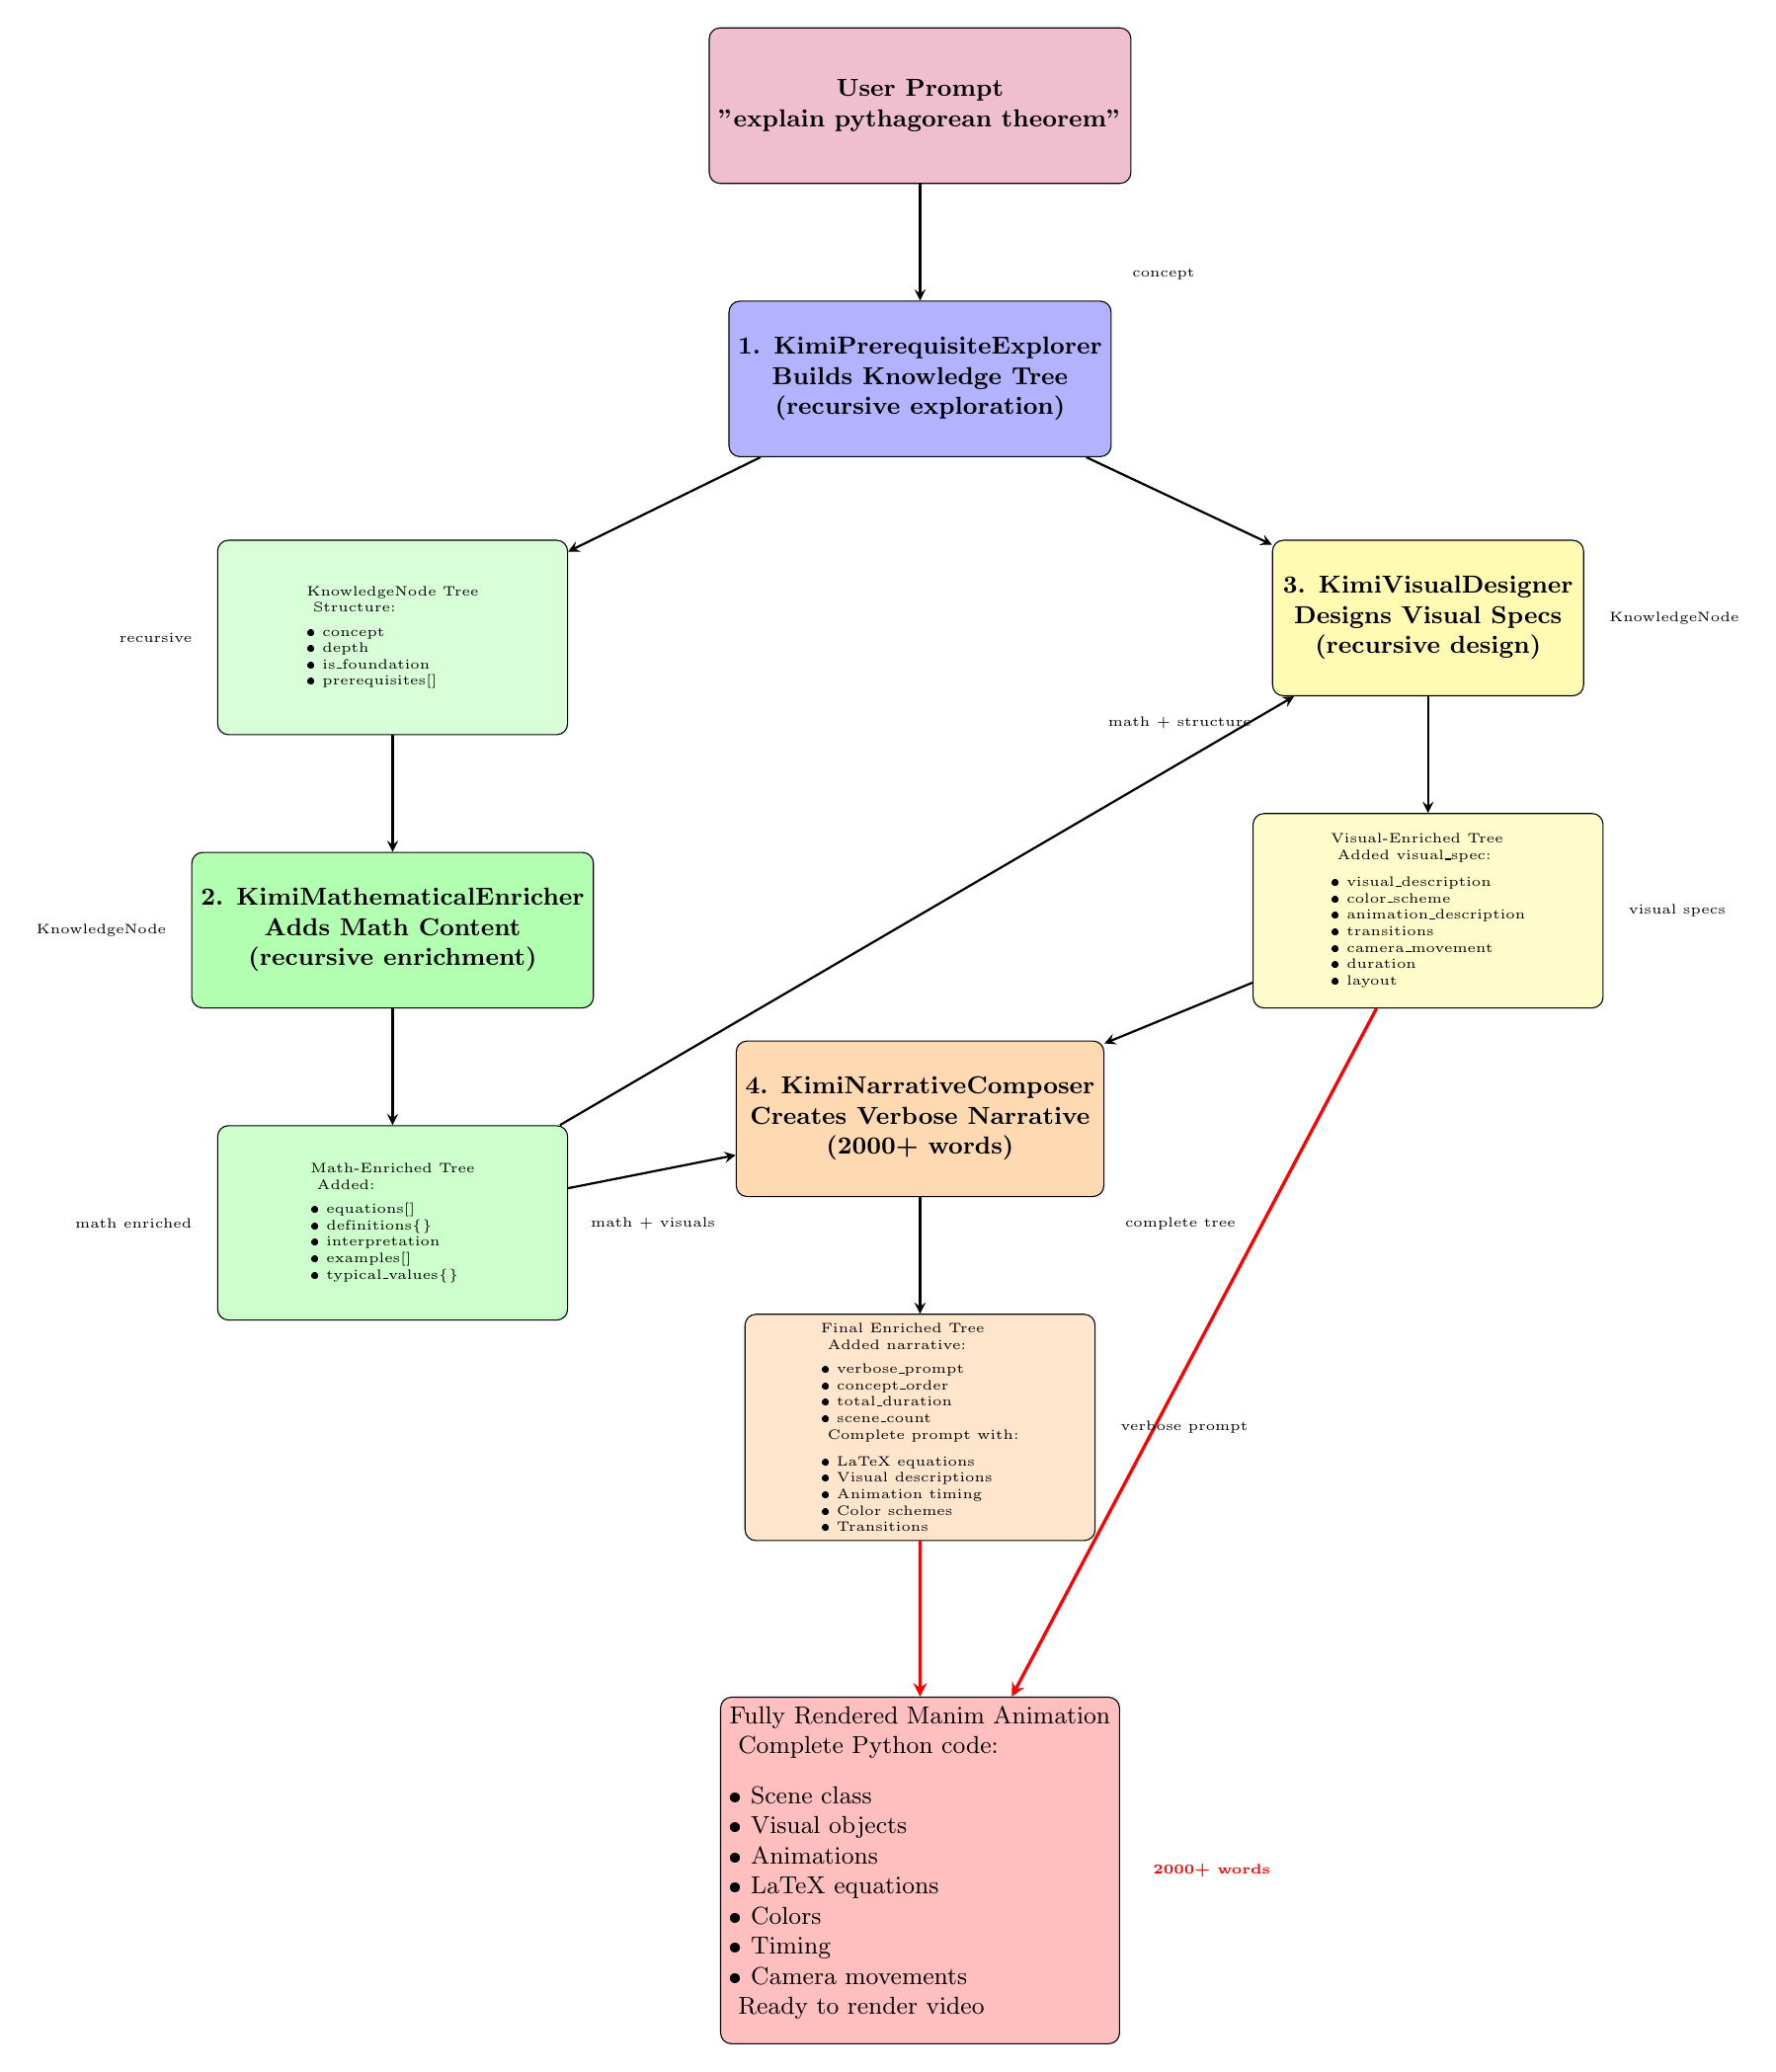
\begin{tikzpicture}[
    node distance=1.5cm,
    agent/.style={rectangle, rounded corners, minimum width=4cm, minimum height=2cm, 
                  text centered, draw=black, fill=blue!25, font=\small\bfseries, align=center},
    data/.style={rectangle, rounded corners, minimum width=4.5cm, minimum height=2.5cm,
                 text centered, draw=black, fill=green!20, font=\tiny, align=left},
    output/.style={rectangle, rounded corners, minimum width=5cm, minimum height=3cm,
                   text centered, draw=black, fill=orange!25, font=\small, align=left},
    arrow/.style={->, >=stealth, thick, black}
]

% Input
\node[agent, fill=purple!25] (input) at (0,0) {
    User Prompt\\
    "explain pythagorean theorem"
};

% Stage 1: Prerequisite Explorer
\node[agent, fill=blue!30, below=of input] (explorer) {
    1. KimiPrerequisiteExplorer\\
    Builds Knowledge Tree\\
    (recursive exploration)
};

% Tree output
\node[data, fill=green!15, below left=of explorer, xshift=-1cm] (tree1) {
    KnowledgeNode Tree\\
    \vspace{0.1cm}
    Structure:\\
    • concept\\
    • depth\\
    • is\_foundation\\
    • prerequisites[]
};

% Stage 2: Mathematical Enricher
\node[agent, fill=green!30, below=of tree1] (math) {
    2. KimiMathematicalEnricher\\
    Adds Math Content\\
    (recursive enrichment)
};

% Math-enriched tree
\node[data, fill=green!20, below=of math] (tree2) {
    Math-Enriched Tree\\
    \vspace{0.1cm}
    Added:\\
    • equations[]\\
    • definitions\{\}\\
    • interpretation\\
    • examples[]\\
    • typical\_values\{\}
};

% Stage 3: Visual Designer
\node[agent, fill=yellow!30, below right=of explorer, xshift=1cm] (visual) {
    3. KimiVisualDesigner\\
    Designs Visual Specs\\
    (recursive design)
};

% Visual-enriched tree
\node[data, fill=yellow!20, below=of visual] (tree3) {
    Visual-Enriched Tree\\
    \vspace{0.1cm}
    Added visual\_spec:\\
    • visual\_description\\
    • color\_scheme\\
    • animation\_description\\
    • transitions\\
    • camera\_movement\\
    • duration\\
    • layout
};

% Stage 4: Narrative Composer
\node[agent, fill=orange!30, below=of explorer, yshift=-6cm] (narrative) {
    4. KimiNarrativeComposer\\
    Creates Verbose Narrative\\
    (2000+ words)
};

% Final enriched tree
\node[data, fill=orange!20, below=of narrative] (tree4) {
    Final Enriched Tree\\
    \vspace{0.1cm}
    Added narrative:\\
    • verbose\_prompt\\
    • concept\_order\\
    • total\_duration\\
    • scene\_count\\
    \vspace{0.1cm}
    Complete prompt with:\\
    • LaTeX equations\\
    • Visual descriptions\\
    • Animation timing\\
    • Color schemes\\
    • Transitions
};

% Final Output: Manim Code
\node[output, fill=red!25, below=of tree4, yshift=-0.5cm] (manim) {
    Fully Rendered Manim Animation\\
    \vspace{0.2cm}
    Complete Python code:\\
    • Scene class\\
    • Visual objects\\
    • Animations\\
    • LaTeX equations\\
    • Colors\\
    • Timing\\
    • Camera movements\\
    \vspace{0.2cm}
    Ready to render video
};

% Flow arrows
\draw[arrow] (input) -- (explorer);
\draw[arrow] (explorer) -- (tree1);
\draw[arrow] (tree1) -- (math);
\draw[arrow] (math) -- (tree2);
\draw[arrow] (tree2) -- (visual);
\draw[arrow] (explorer) -- (visual);
\draw[arrow] (visual) -- (tree3);
\draw[arrow] (tree3) -- (narrative);
\draw[arrow] (tree2) -- (narrative);
\draw[arrow] (narrative) -- (tree4);
\draw[arrow, red, very thick] (tree4) -- (manim);
\draw[arrow, red, very thick] (tree3) -- (manim);

% Labels on arrows
\node[font=\tiny, above right=0.2cm of explorer] {concept};
\node[font=\tiny, left=0.2cm of tree1] {recursive};
\node[font=\tiny, left=0.2cm of math] {KnowledgeNode};
\node[font=\tiny, left=0.2cm of tree2] {math enriched};
\node[font=\tiny, below left=0.2cm of visual] {math + structure};
\node[font=\tiny, right=0.2cm of visual] {KnowledgeNode};
\node[font=\tiny, right=0.2cm of tree3] {visual specs};
\node[font=\tiny, below right=0.2cm of narrative] {complete tree};
\node[font=\tiny, below left=0.2cm of narrative] {math + visuals};
\node[font=\tiny, right=0.2cm of tree4] {verbose prompt};
\node[font=\tiny\bfseries, right=0.3cm of manim, text=red] {2000+ words};

\end{tikzpicture}
\end{document}
